\documentclass[10pt,twocolumn]{article}
\usepackage[letterpaper,margin=0.72in,columnsep=0.25in]{geometry}
\usepackage[T1]{fontenc}
\usepackage{lmodern}
\usepackage{amsmath,amssymb,booktabs,graphicx,microtype}
\usepackage{xcolor,tikz}
\usetikzlibrary{arrows.meta,positioning,fit,calc}
\usepackage[hidelinks]{hyperref}
\usepackage{url,flushend}
\hypersetup{pdftitle={MR-NWM: Language-Model-Centered World Models for Multimodal, Multi-Rate RAN Control},pdfauthor={},pdfsubject={Research preprint and reproducible synthetic benchmark},pdflang={en-US}}
\setlength{\parindent}{1em}
\setlength{\parskip}{0pt}
\setcounter{dbltopnumber}{3}
\renewcommand{\dbltopfraction}{0.85}
\newcommand{\R}{\mathbb{R}}
\newcommand{\E}{\mathbb{E}}
\newcommand{\sg}{\operatorname{stopgrad}}
\title{\vspace{-1.4em}MR-NWM: Language-Model-Centered World Models\\for Multimodal, Multi-Rate RAN Control}
\author{}
\date{Research preprint, October 2026}

\begin{document}
\maketitle
\begin{abstract}
MR-NWM is a language-model-centered architecture for multimodal, multi-rate
radio access network (RAN) world modeling. A pretrained language transformer
serves as the shared slow backbone. Continuous modality adapters receive
state/traffic sequences, real/imaginary CSI and IQ features, topology nodes,
and optional patch features, with explicit observation ages and sampling
periods. Two causal views of the same language backbone separate operational
preferences from exogenous physical evidence. A context-conditioned recurrent
subnetwork then predicts numerical state transitions at the fast rate using a
cached modulation packet, with optional slow/fast physics-expert sharing.
We supply this pretrained-model integration alongside a lightweight,
train-from-scratch reference variant. Three-seed, eight-variant measurements on
a fully specified two-link queue/interference simulator evaluate only the
lightweight variant: dynamics, distribution shift, controlled-language parsing,
action effects, decision regret, and host-observed timing. A separate Stage-A
check trains a small LSTM forecaster on the public 5G-IANA UC6 real 5G
measurement campaign (26{,}733 one-second KPI records, no control log) and
measures four-second KPI forecasts against persistence on chronologically
later sessions: throughput, RTT, and RSRQ improve by 31--43\% NMSE while RSRP,
nearly constant at this horizon, is forecast worse than persistence. Those
results do not establish performance of a trained language-foundation RAN
model. The project provides executable multimodal/gradient/causality tests and
a reproducible path from the small reference experiment and the real-data
forecast check toward the intended language-based system, without claiming
calibrated radio behavior or deterministic real-time deadlines.
\end{abstract}

\section{Introduction}
Network operators express objectives in terms of service quality, energy,
reliability, and business priorities. A controller must translate these
objectives into measurable quantities, evaluate candidate actions against
network dynamics, and respect actuator and timing constraints. Language models
can provide an extensible interface to these tasks, while continuous-valued
predictors can represent the physical consequences of actions without
converting every measurement into text.

Two broad designs are possible: a common multimodal backbone can process
language and network measurements, or a semantic component can invoke a
separate dynamics model. Neither design inherently determines the numerical
representation of wireless observations. In particular, a language-derived
backbone can receive continuous embeddings, and a tool interface can transmit
continuous tensors. Nor does a modular interface necessarily prohibit joint
training: differentiability depends on the operations and training graph.
The relevant questions are therefore empirical: what should be shared, which
information should influence the transition law, and how should computational
work be divided across rates?

The full MR-NWM architecture places a pretrained language model at the center
of slow multimodal fusion and intent processing. Its numeric adapters and fast
physical subnetwork are jointly trainable around that backbone. The lightweight
reference hypothesis is that a slow context encoder and a small recurrent
transition operator can be coupled through weight sharing and low-dimensional
conditioning, while keeping intent-to-objective compilation explicit.
This construction builds on established multi-rate recurrence, hypernetworks,
feature modulation, and low-rank parameterization
\cite{koutnik2014,ha2016,perez2018,hu2022}. We do not claim these components
individually as new. The contribution of this reference study is their concrete
composition with an enforced preference/dynamics boundary and an evaluation
protocol that can falsify benefits from sharing or gradient coupling.

The implementation makes three choices that are particularly consequential.
First, continuous physical state and exogenous context enter through numeric
encoders rather than text quantization. Second, the slow physical stream cannot
read preference tokens, including through the recurrent expert. Third, a
forecast spanning two macro windows passes its predicted terminal state and
fast summary into the next window. Thus long-horizon errors cannot be hidden by
resetting the initial condition. These choices are independently covered by
regression tests.

\input{language_foundation.tex}

\section{Related Work and Scope}
World models learn action-conditioned transitions for prediction and planning;
DreamerV3 is an influential example of learning control through a latent world
model across diverse environments \cite{hafner2023}. MR-NWM is a supervised
prediction and finite-candidate auditing study. It does not implement Dreamer,
learn an actor, or demonstrate reinforcement-learning performance.

Clockwork recurrent networks demonstrate that recurrent computation can be
partitioned by update frequency \cite{koutnik2014}. HyperNetworks generate
parameters for another network \cite{ha2016}; FiLM conditions computation with
feature-wise affine transformations \cite{perez2018}. LoRA parameterizes an
update using low-rank factors \cite{hu2022}. Here the low-rank factors are
generated from each macro context, while the base model is also trained.
This differs from the standard frozen-backbone fine-tuning setup of LoRA.

Input-dependent state-space models motivate selective recurrent memory
\cite{gu2023}. Our physics expert is a simple gated recurrence, with bounded
forgetting coefficients. It is neither an implementation of Mamba nor a
physics-constrained channel model. Similarly, the heterogeneous expert mixture
executes every expert and therefore offers no sparse-MoE compute saving.

Flow matching regresses a vector field along a prescribed probability path
\cite{lipman2023}. Transfusion provides an example of combining discrete and
continuous objectives in one multimodal model \cite{zhou2024}. We include an
optional action-conditioned flow head for future stochastic trajectory studies,
but the reported deterministic benchmark does not use it. In particular, no
claim about improved uncertainty calibration follows from its presence.

The repository has two explicit realizations. The language-foundation path
loads an external pretrained transformer and tokenizer and adds numeric/graph
adapters. The lightweight benchmark path uses randomly initialized semantic
MLPs, with no pretrained language weights. No over-the-air measurements, RIC
integration, or DU deployment are supplied. The controlled-language benchmark
cannot support open-domain or foundation-model zero-shot claims.

\section{Problem Formulation}
\subsection{State, actions, context, and intent}
Let $s_t\in\R^{d_s}$ denote the observable network state, $a_t\in\R^{d_a}$ a
candidate action, and $c_T\in\R^{d_c}$ measured exogenous context for macro
window $T$. Each window contains $K$ micro steps. Operational intent $I_T$
determines objective weights $w(I_T)$ and, in a fuller system, explicit
constraints. A causal transition model has the form
\begin{equation}
 s_{t+1}=F(s_t,a_t,c_T,\epsilon_t),\qquad
 U_t=w(I_T)^\top\psi(s_{t+1},a_t).
 \label{eq:causal}
\end{equation}
The preference part of an intent does not directly enter $F$. If a language
input reports an external event or a configuration change that affects
dynamics, that information must be extracted into a distinct, validated
context variable. If an intent changes the policy, it can of course change the
realized future \emph{through actions}. Equation~\eqref{eq:causal} concerns
predictions under the same intervened action sequence and context.

This separation gives a testable invariant:
\begin{equation}
 \hat{s}_{1:H}(I,a_{0:H-1},c,s_0)
 =\hat{s}_{1:H}(I',a_{0:H-1},c,s_0).
 \label{eq:invariant}
\end{equation}
The reference simulator satisfies this invariant by construction. A physical
event described in text is not interchangeable with an optimization preference;
keeping them in a single undifferentiated prompt would make the intended causal
semantics ambiguous.

\subsection{Time scales and placement}
Our notation describes computational rates, not measured radio deadlines.
The O-RAN architecture specifies Near-RT RIC control loops on the order of
10~ms to 1~s and permits faster control inside E2 nodes; loop timing is use-case
dependent \cite{oran2026}. A sub-millisecond fast model is a possible engineering
target for selected functions, rather than a consequence of assigning a module
to a DU. Likewise, $K$ is a modeling hyperparameter here; no micro-step in the
toy simulator is calibrated to a transmission interval.

\subsection{World model, planner, and optional policy}
\label{sec:planner-actions}
An action-conditioned world model predicts consequences; a planner selects
actions; a policy network amortizes that selection. These are distinct objects.
For partially observed deployments, let $h_t$ contain only observations available
by decision time, their ages, and previous applied actions. The proposed
transition model is $F_\theta(\cdot\mid h_t,\bar a_t,c_T,\Delta_t)$, where
$\bar a_t$ is the action that actually takes effect and $\Delta_t$ is its
duration. A requested action can be rejected, delayed, or clipped, and must not
silently replace $\bar a_t$ in a training record. A receding-horizon planner would
solve
\begin{equation}
 A^* = \arg\max_{A\in\mathcal A(h_t)}
 \E_{F_\theta}\!\left[\sum_{k=0}^{H_p-1}\gamma^k
 U(\hat s_{t+k+1},a_{t+k};w_T)\right],
 \label{eq:planner-contract}
\end{equation}
Here $H_p$ is the planning horizon, $\gamma\in[0,1]$ a discount factor, and
$\mathcal A(h_t)$ the feasible candidate-sequence set. The search respects
actuator limits, service constraints, and a fixed computation budget.
Only its first accepted action is executed before replanning from new evidence.
Finite enumeration, sampling, or model predictive control can implement this
planner without training an actor. An optional actor
$\pi_\phi(a\mid h_t,w_T)$ can later be trained from evaluated planner decisions
or by reinforcement learning. Historical operator actions are behavior samples,
not automatically optimal-action labels.

Equation~\eqref{eq:planner-contract} is a deployment contract, not a reported
closed-loop result. The implemented \texttt{planning\_audit} ranks a finite grid
of two-link power vectors by \emph{one-step} utility. It repeats each candidate
over the forecast call but scores only its first predicted state; it neither
searches general action sequences nor trains an actor.

\subsection{A bounded, hierarchical RAN action space}
Table~\ref{tab:planner-actions} identifies actuators rather than listing KPIs
as actions. A slow controller can choose slice budgets, scheduler modes, and
power envelopes; a local controller realizes the corresponding fast allocations.
The same actuator must have one owner per control interval. The planner may
change only fields exposed by the selected simulator or execution interface;
capability masks disable unsupported actions. Neither the slow language backbone
nor a nominal model step implies permission to perform slot-level scheduling
through a Near-RT RIC. Placement and deadlines require a separate integration
measurement~\cite{oran2026}.

\begin{table*}[t]
\centering
\small
\caption{Proposed RAN action contract. Only the first row is exercised in the
current synthetic decision audit. The other rows define scoped extensions,
not implemented or experimentally validated capabilities. Rates describe
ownership and dependencies, not measured execution deadlines.}
\label{tab:planner-actions}
\begin{tabular}{p{0.15\textwidth}p{0.27\textwidth}p{0.25\textwidth}p{0.23\textwidth}}
\toprule
Action family & Decision variables & Rate and required evidence & Essential limits \\
\midrule
Power / interference & Per-link power or power envelope; current reference uses
two normalized powers & Local fast adjustment under slower envelopes;
applied power, channel/interference, load & Total/per-link power, ramp rate,
neighbor interference \\
Resources / scheduling & Slice PRB or RBG budget; scheduler mode; optionally local
UE allocations & Budgets/modes at a supervisory rate; local scheduling faster;
queue, traffic, CQI, granted resources & Resource conservation, minimum service,
integer allocations, one actuator owner \\
Beam management & Codebook beam, candidate set, sweep/measurement trigger &
Channel/blockage dependent; beam powers, alignment, switching feedback & Valid
codebook, switching and measurement overhead \\
Mobility / association & Target cell, handover trigger or parameters, association &
Event driven; neighbor measurements and handover outcomes & Dwell/hysteresis,
interruption cost, reachable target \\
Admission / energy & Admit or defer traffic; carrier/cell sleep and wake &
Load driven, with slower activation effects; demand and energy measurements &
Coverage, wake delay, service obligations \\
Measurement / reporting & Measurement period, report rate, sensor activation &
Information refresh at multiple rates; observation ages, acquisition cost &
Maximum staleness and acquisition budget; model the changed observation process \\
\bottomrule
\end{tabular}
\end{table*}

Throughput, delay, and energy are outcomes or objective terms, not directly
commandable actions. External traffic, mobility, and channel evolution are
exogenous unless a particular task explicitly controls them. Objective weights
are policy configuration, not physical interventions. Selecting a model,
refreshing context, or requesting replanning is a supervisory operation; it is
not evidence that a radio action was applied. Edge offloading and cache placement
would require additional compute/cache state and actuators and are outside this
paper's evaluated action space. Every extension also needs an explicit
hold/fallback behavior; zero transmit power is not a universal safe fallback.

\subsection{What public data can supervise}
\label{sec:action-data}
The absence of action logs in UC6 and UCC production traces does not imply that
all public wireless datasets lack action information. Three evidence types
must be separated.

\paragraph{Passive commercial observations.}
UC6 and UCC support observation forecasting, as evaluated in
Section~\ref{sec:uc6}. They do not provide the applied RAN control and effective
time needed to identify power or resource interventions. Unknown actions must
be masked rather than encoded as zero power.

\paragraph{Measured alternatives for beam selection.}
DeepSense task releases include measured beam-power vectors and best-beam
indices derived from them~\cite{deepsensebeam}. These can supervise beam
selection and, with a matched evaluation target, ranking loss relative to the
measured best beam. An index derived by taking an argmax is not an executed
control trajectory. Beam sweeps alone do not identify queue evolution,
handover interruption, or the long-term effects of changing beams. The measured
power vector must be a target rather than an unavailable decision-time input.

\paragraph{Configuration-conditioned RF-emulator experiments.}
The public Colosseum COMMAG and ColO-RAN releases document slicing allocations
and RR/WF/PF scheduling configurations~\cite{commagdata,colorandata}.
Our source audit on 29 October 2026 downloaded one per-UE CSV from each release
and found timestamp, \texttt{slice\_prb}, \texttt{scheduling\_policy},
\texttt{power\_multiplier}, queue, CQI, throughput, and requested/granted-resource
fields. Both inspected files contain a single resource configuration,
scheduler mode, and power multiplier; a column's presence is not evidence of
intervention coverage. The COMMAG README describes a resizing schedule, but
that schedule cannot substitute for changes observed in a particular CSV.
The source revisions, sample paths, hashes, and findings are recorded in the
repository's action-data audit.

Commercial Traffic Twinning provides a complementary collection: a
one-BS/eight-UE Colosseum experiment replays commercial traffic under five
slice-resource configurations and two scheduling modes, with timestamped
PHY/MAC/application measurements~\cite{twinning2024}. Those interventions and
feedback occur in the RF emulator; the commercial origin of the offered traffic
does not make the resulting action-response trajectories production-network
interventions. Its published MAC counters aggregate over 250~ms and do not
recover individual slot allocations. This audit inspected its documentation,
not its full data archives.

These releases are candidates for \emph{restricted}, configuration-conditioned
training after entity, unit, timing, coverage, and license checks. Constant-action
runs can teach within-configuration responses, but do not alone identify
switching transients or arbitrary multistep control. Resource demand and grants
aggregated during an interval are not automatically decision-time actions.
Trial identifiers or future KPI windows must not leak into planner inputs.
None of these releases has been used to train the models reported here, and
none establishes a complete, jointly observed action space for Table~\ref{tab:planner-actions}.

\subsection{Closing action-coverage gaps with controlled simulation}
For the broad sequential-control extension, our proposed data route combines
measured representations and restricted public control experiments with
\emph{explicitly labeled} simulator interventions. Simulation is not necessary
for every task: measured beam-selection supervision already exists. It is a
practical source of missing action coverage and switching outcomes when
corresponding controlled measurements are unavailable.

The first extension should retain power control as a synthetic regression
test and separately study slice budgets plus scheduler selection in a
packet-level environment. It should not claim simultaneous validation of
beams, handovers, energy, and admission. ns-3/5G-LENA offers channel, queue,
scheduler, traffic, and power-control components~\cite{lena2026}; the chosen
version still needs task-specific actuator hooks and logging. A propagation
or ray-tracing model alone does not generate scheduler/queue feedback.

Each episode should preserve available observation history, exogenous inputs,
requested and applied actions, effective times and durations, execution status,
subsequent independently computed KPI/cost measurements, behavior policy,
simulator version, seeds, and provenance. Collect rule-based and varied
feasible policies, not only an expert's preferred actions. From a saved simulator
state, replay alternatives with matched exogenous realizations to measure action
effects, retaining the shared branch origin for grouped train/test splitting.
Fit action-conditioned dynamics first; evaluate a bounded search planner next;
distill an actor only if search latency justifies it. Report multistep error,
action-ranking regret, realized return, service violations, switching costs,
and total decision latency against rules and an action-independent predictor.
Use held-out scenarios and independently acquired testbed/field feedback before
claiming transfer. LLMs may propose traffic scenarios or constraints, but the
simulator or instrumented network must compute physical outcomes. Synthetic,
RF-emulator, derived-label, and field evidence remain separate throughout.


\section{Lightweight Reference Variant and Training}
\subsection{Slow heterogeneous mixture}
At each macro step, token embeddings for intent, a state projection, a context
projection, and the previous fast summary form
\begin{equation}
 Z_T=[E_I(I_T);E_s(s_{T,0});E_c(c_T);H_{T-1}].
\end{equation}
The intent tokenizer is fitted only to the controlled training corpus. Learned
positions are added to intent tokens; physical token types have their own
encoders. A single attention block produces $h_i$, followed by a dense mixture
of one semantic MLP expert $E_{\rm sem}$ and one recurrent expert
$E_{\rm phy}$. For a modality indicator $m_i$,
\begin{align}
 \pi_i &=\operatorname{softmax}(W_g[h_i;\operatorname{onehot}(m_i)]),\\
 y_i &=\pi_{i,\rm sem}E_{\rm sem}(h_i)
       +\pi_{i,\rm phy}E_{\rm phy}(h_i).
\end{align}
For intent tokens the physics term is the identity, and the recurrent physics
expert starts afresh at the first physical token. Physical attention queries
are masked from intent keys. Both restrictions are necessary: attention masking
alone would still allow a recurrent expert to carry semantic information into
physical tokens. The semantic stream may read the physical context.

The mean physical output gives $h_T^p$. A masked mean over intent outputs gives
$h_T^I$, and a head predicts
$\hat w_T=\operatorname{softmax}(W_I h_T^I)$ over throughput, queue, and energy
features. The router is weakly regularized by
\begin{equation}
 \mathcal L_{\rm route}=-\frac{1}{|\mathcal V|}
 \sum_{i\in\mathcal V}\log\pi_{i,m_i},
\end{equation}
where $\mathcal V$ excludes padding. This encourages modality specialization;
it does not establish that the experts learn interpretable physical laws.

\begin{figure*}[t]
\centering
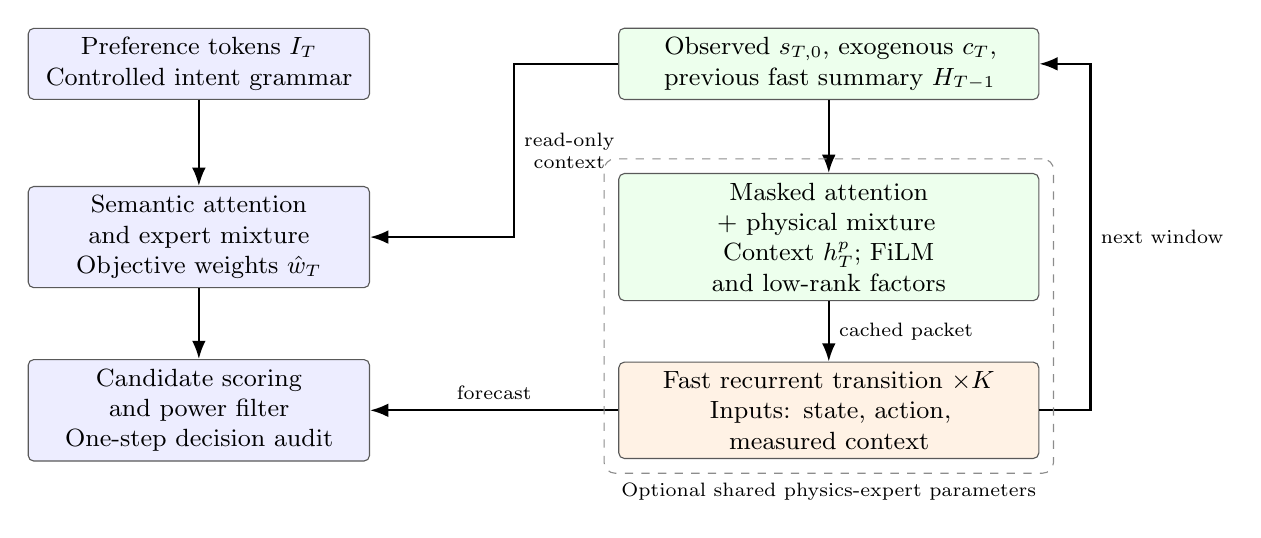
\begin{tikzpicture}[
 font=\small,>=Latex,
 box/.style={draw=black!65,rounded corners=2pt,align=center,minimum height=0.85cm},
 arr/.style={->,thick},node distance=0.45cm]
 \node[box,fill=blue!7,text width=4.1cm] (intent) at (0,2.6)
 {Preference tokens $I_T$\\Controlled intent grammar};
 \node[box,fill=green!7,text width=5.1cm] (physical) at (8,2.6)
 {Observed $s_{T,0}$, exogenous $c_T$,\\previous fast summary $H_{T-1}$};
 \node[box,fill=blue!7,text width=4.1cm] (sem) at (0,0.4)
 {Semantic attention\\and expert mixture\\Objective weights $\hat w_T$};
 \node[box,fill=green!7,text width=5.1cm] (slow) at (8,0.4)
 {Masked attention + physical mixture\\Context $h_T^p$; FiLM and low-rank factors};
 \node[box,fill=orange!10,text width=5.1cm] (fast) at (8,-1.8)
 {Fast recurrent transition $\times K$\\Inputs: state, action, measured context};
 \node[box,fill=blue!7,text width=4.1cm] (utility) at (0,-1.8)
 {Candidate scoring\\and power filter\\One-step decision audit};
 \draw[arr] (intent) -- (sem);
 \draw[arr] (physical) -- (slow);
 \draw[arr] (physical.west) -- (4,2.6) -- node[right,align=center,font=\scriptsize]
 {read-only\\context} (4,0.4) -- (sem.east);
 \draw[arr] (sem) -- (utility);
 \draw[arr] (slow) -- node[right,font=\scriptsize] {cached packet} (fast);
 \draw[arr] (fast) -- node[above,font=\scriptsize] {forecast} (utility);
 \draw[arr] (fast.east) -- ++(0.65,0) |- node[pos=0.25,right,font=\scriptsize]
 {next window} (physical.east);
 \node[draw=black!45,dashed,rounded corners,fit=(slow)(fast),inner sep=0.18cm,
 label={[font=\scriptsize]below:Optional shared physics-expert parameters}] {};
\end{tikzpicture}
\caption{Lightweight reference-variant information flow. Physical prediction has no path from preference
tokens. The semantic stream can use physical observations; numerical action evaluation
uses the forecast and compiled objectives. Slow and fast execution are separated in the
API, while shared training parameters remain a research option.}
\label{fig:architecture}
\end{figure*}

\subsection{Fast recurrence and modulation}
A hyper-projection from $h_T^p$ generates
$(\gamma_T,\beta_T,A_T,B_T)$, with
$\gamma_T=1+0.1\tanh(\cdot)$,
$\beta_T=0.1\tanh(\cdot)$, and bounded factors $A_T,B_T\in\R^{d\times r}$.
Within a macro window, these tensors are held fixed. Each micro step encodes
the current state, candidate action, and measured context:
\begin{equation}
 x_k=\gamma_T\odot\operatorname{SiLU}(W_x[s_k;a_k;c_T])+\beta_T.
\end{equation}
Let $n_k=\operatorname{LN}(x_k)$ and
$(u_k,g_k)=W_{\rm in}n_k$, with a SiLU applied to $u_k$. The physics memory is
\begin{align}
 \alpha_k&=\sigma(W_\alpha u_k),\\
 z_k&=\alpha_k\odot z_{k-1}+
        (1-\alpha_k)\odot\tanh(W_Bu_k),\\
 o_k&=x_k+W_o[W_Cz_k\odot\sigma(g_k)]
           +\frac{n_kA_TB_T^\top}{\sqrt r},\\
 \hat s_{k+1}&=\hat s_k+W_\Delta o_k.
 \label{eq:fast}
\end{align}
The last expression is a residual \emph{state increment}; the measured state is
not replaced by an action-independent macro forecast. Although $z_k$ has a
bounded convex update, this alone does not guarantee stability of the complete
autoregressive predictor or the downstream control loop.

In the shared variant, the slow physical expert and fast recurrence refer to
the identical parameter object. No extra copy is trained. A separately deployed
process would instead receive a versioned copy of the trained parameters;
weight sharing during training does not create cross-machine shared memory.
The unshared variant allocates an independent fast core. All variants retain
explicit dependence on actions and continuous context.

\subsection{Feedback and training graph}
The $K$ fast hidden states are compressed by a kernel-$K$, stride-$K$ one-dimensional
convolution into $H_T$. This summary is available to the \emph{next} macro step.
It cannot contain future observations. Memory $z$ resets at a macro boundary;
information persists through $H_T$ and the terminal predicted state.

Training uses two consecutive macro windows, initialized once with the observed
state. At the boundary,
\begin{equation}
 s_{T+1,0}=\hat s_{T,K},\qquad
 H_T=R(o_{T,1:K}).
\end{equation}
No target state is substituted. Within each macro window, $s_k$ and $z_k$ are
detached every $L=3$ steps. The modulation tensors retain their gradients.
The direct path from each micro-step loss to the slow context therefore remains
available despite truncation. Shared parameters also receive gradients through
the fast recurrence itself. Truncation limits the differentiated history; it
neither proves convergence nor prevents all gradient explosions. We additionally
clip the global gradient norm to one.

With $H=2K$, the reference loss is
\begin{align}
 \mathcal L&=\mathcal L_{\rm dyn}+0.2\mathcal L_I+0.01\mathcal L_{\rm route},\\
 \mathcal L_{\rm dyn}&=\frac{1}{BHd_s}\sum_{b,k,j}
    (\hat s_{b,k,j}-s_{b,k,j})^2,\\
 \mathcal L_I&=-\frac{1}{2B}\sum_{b,T,j}w_{b,j}\log\hat w_{b,T,j}.
\end{align}
Semantic targets are determined by the actual words in each training phrase.
There is no independently sampled next-token target and no claim of language
model pretraining. The optional flow loss is disabled for all reported runs.

For a controlled gradient ablation, the detached variant uses an independent
fast core and $\sg(h_T^p)$ before its modulator. The modulator, fast core,
semantic head, and route loss remain trainable. Comparing this variant with
the \emph{unshared} jointly trained model isolates the bridge-gradient choice.
Comparing it only with the shared model would also change parameter sharing.

\subsection{Optional probabilistic trajectory head}
For an optional extension, let $y=s_{T,1:K}$ and
$\xi\sim\mathcal N(0,I)$. A velocity network conditioned on both $h_T^p$ and the
\emph{candidate action sequence} minimizes
\begin{equation}
 \E_{\tau,\xi}\big\|v_\phi((1-\tau)\xi+\tau y,\tau,h_T^p,a_{0:K-1})
                         -(y-\xi)\big\|^2.
\end{equation}
The sampling API requires an explicit base draw and integrates the velocity
using Euler steps. Starting every sample at zero would not reproduce the
Gaussian-base generative model. The optional output is separate from
Equation~\eqref{eq:fast}; it is not silently injected into the deterministic
rollout. We test differentiation and sampling reproducibility, while leaving
probabilistic accuracy and calibration for a dedicated study.

\section{Reproducible Evaluation Protocol}
\label{sec:protocol}
\subsection{Normalized two-link environment}
The state contains two link gains $g$, two queues $q$, and two interference
variables $j$. Actions are two normalized powers $p\in[0,1]^2$; context contains
arrival rates $\lambda_1,\lambda_2$, cross-coupling $\chi$, and mobility $\mu$.
For each link $i$, with $\bar i$ its neighbor,
\begin{align}
 g'_{i}&=\operatorname{clip}((1-\mu)g_i+0.55\mu+\epsilon_i,0.05,1.2),\\
 r_i&=\log_2\left(1+\frac{4g_ip_i}{0.2+j_i+\chi p_{\bar i}}\right),\\
 q'_i&=\operatorname{clip}(q_i+\lambda_i-0.12r_i,0,2),\\
 j'_i&=0.65j_i+0.35\chi p_{\bar i},
\end{align}
where $\epsilon_i\sim\mathcal N(0,0.005^2)$. Powers are independently sampled
uniformly on $[0,1]$. Initial gains, queues, and interference are uniformly
sampled from $[0.2,0.9]$, $[0.1,0.9]$, and $[0.05,0.25]$, respectively.
Training context uses $\lambda_i\sim U(0.05,0.15)$,
$\chi\sim U(0.08,0.25)$, and $\mu\sim U(0.03,0.12)$.
The joint shift adds $0.12$, $0.30$, and $0.25$ to those variables, respectively.
Thus OOD context values for coupling and mobility do not overlap training.

The system has controllable queues and delayed interference, but no waveform,
antenna array, coding, beam management, scheduler, packet simulator, or calibrated
propagation model. It is an intentionally small system-identification test.
The coefficients and state normalization are synthetic choices; they must not
be interpreted as measurements of a mobile network.

\subsection{Intent splits and decision audit}
Three objective names---throughput, latency, and energy---are used in singleton
and two-objective phrases. A target puts equal weight on the named objectives.
Three training templates vary the wording. Two held-out templates reorder the
same known words. An additional test uses all three objectives together, a
combination absent during training. No model or tokenizer is fitted to these
test phrases. Because this is a deliberately constrained grammar, its scores
measure compositional parsing under that grammar, not open-language zero-shot
generalization.

For each test state we also enumerate powers from
$\{0.1,0.4,0.7\}^2$, retaining only candidates with
$p_1+p_2\leq0.8$. The utility features are normalized post-transition rate,
negative mean queue, and negative mean power. The learned model chooses a
candidate using predicted features and inferred weights. We measure the regret
against the exact simulator's best \emph{feasible candidate}, evaluated with
the true intent weights. A second regret calculation substitutes the true
weights into model selection to isolate prediction error from parsing error.
The audit is deterministic and one step long; it is not a learned policy or
an end-to-end closed-loop control experiment. Zero power violations are an
expected property of the candidate filter, not evidence of learned safety.

\subsection{Baselines and matched comparisons}
The eight executable variants are: shared MR-NWM; unshared MR-NWM; shared MR-NWM
without FiLM or low-rank modulation; the unshared detached-bridge control; an
action/context-conditioned residual MLP; an approximately parameter-matched MLP;
a standalone recurrent model; and persistence. The MLPs have two hidden layers
of width 64 and 160, respectively, and predict the same state increments. They have no
semantic parser, so semantic scores are not invented for that baseline.
The standalone recurrent control uses the same fast recurrence and truncation
schedule as MR-NWM, with no slow tier or modulation. Parameters and optimization
steps are reported rather than claiming exact compute matching. No pure LLM,
pretrained wireless foundation model, or
industrial controller is represented by a synthetic row in a table.

All trainable variants use 300 AdamW updates, batch size 48, learning rate 0.002,
and weight decay $10^{-4}$. MR-NWM uses width 32, recurrent state size 16, rank 2,
four attention heads, and $K=5$. All models receive identical training
trajectories, indexed by seeds $100000+u$ for update $u$. Initialization seeds
are 11, 22, and 33. Evaluation uses 256 trajectories per split with seed
900000, never used for training. Models are evaluated after the fixed final
update; no test score selects a checkpoint or changes the budget.

\subsection{Metrics and timing}
We use signal-energy NMSE,
\begin{equation}
 10\log_{10}\frac{\sum_{b,k,j}(\hat s_{b,k,j}-s_{b,k,j})^2}
                      {\sum_{b,k,j}s_{b,k,j}^2},
\end{equation}
with lower values better. This is distinct from dividing MSE by centered
target variance. Per-step MSE and per-state NMSE accompany the aggregate,
since a global score can hide errors in small-scale variables. A paired action
audit compares the predicted trajectory difference under $a$ and $1-a$ with
the noise-free simulator difference. A predictor ignoring actions has zero
effect and therefore an action-effect NMSE of 0~dB.

Intent parsing uses total variation distance
$\tfrac12\|\hat w-w\|_1$ and cosine similarity. Cosine is not converted into
an invented ``alignment percentage.'' For latency, the model is in inference
mode; measurements use ten warm-up calls followed by 100 timed batch-one calls,
with device synchronization around timed regions. We retain raw timing samples
and report p50, p95, and p99. The fast measurement uses a cached modulation packet
and a supplied recurrent state. It excludes slow encoding, data acquisition,
transport, scheduling, model loading, and actuator execution. It therefore
cannot establish a radio control deadline or a deterministic worst-case bound.

\section{Results and Interpretation}
\begin{table*}[t]
\centering
\caption{Measured signal-energy NMSE over ten consecutive forecast steps. Values are
mean $\pm$ sample standard deviation over three initialization seeds. All rows
use the same held-out physical trajectories for a given dynamics split.}
\label{tab:results}
\input{results.tex}
\end{table*}

\begin{figure*}[t]
\centering
\includegraphics[width=0.92\textwidth]{figures/rollout_error.pdf}
\caption{Measured forecast error by horizon. The dotted boundary separates two
five-step macro windows; the second window starts from the model's first-window
terminal prediction. Curves average three initialization seeds. Raw per-seed
curves and per-state NMSE are retained in the result manifest.}
\label{fig:error}
\end{figure*}

\begin{table*}[t]
\centering
\caption{Controlled-vocabulary parsing and finite-candidate decision audit. Lower is
better for all three metrics. Composition refers to the held-out three-objective
combination; it is not a foundation-model zero-shot benchmark.}
\label{tab:intent}
\input{intent_results.tex}
\end{table*}

\input{discussion.tex}

\section{Real-Measurement Stage-A Checks}
\label{sec:uc6}
To probe the pipeline against physically measured data, we run an
observation-forecasting stage on the public 5G-IANA UC6 campaign~\cite{uc6dataset}
(Zenodo record
10037164, CC~BY~4.0): 26{,}733 one-second records of throughput, RTT, RSRQ, and
RSRP between a Nokia edge server and a vehicle-mounted OBU near Ulm, with GPS
position. The campaign contains no control-action log, so this stage
deliberately excludes action conditioning and the language/intent path; it
exercises only data ingestion, cleaning, real-time windowing, and multi-step
KPI forecasting.

Rows are split into trajectory segments at time gaps above 60~s or GPS jumps
above 250~m, yielding 96 segments of which 52 are usable. Missing KPI samples
(21 throughput, 7{,}310 RSRQ/RSRP) are linearly interpolated within segments
and tracked by validity masks; duplicate-second records are ordered, and
glitched positions are repaired before deriving speed and heading context.
Windows use 8~s of history and a 4~s horizon on the native one-second grid.
Splitting is by whole segment in chronological order (70/15/15\%): overlapping
windows never cross the train/evaluation boundary, and test windows come from
physically later measurement sessions. Normalization statistics are fit on
training segments only. This yields 16{,}312 training, 3{,}639 validation, and
6{,}149 test windows.

The forecaster is a deliberately small LSTM (hidden width 64, one layer,
19{,}344 parameters) over the normalized KPI history, with a linear mobility
context gate (position, heading, speed) and a linear decoder producing the
normalized 4-step KPI forecast. It is trained with Adam (learning rate
$10^{-3}$, batch 128, 2{,}000 updates) under a masked MSE loss; the identical
protocol runs for initialization seeds 11, 22, and 33. The baseline is
persistence, i.e., repeating the last observed value. Because persistence is
deterministic given the data, its seed-to-seed standard deviation is exactly
zero. Training ran on an Ascend~910B NPU host; each seed completes in about
21~s. Metrics are computed only at observed target positions, in physical
units.

Table~\ref{tab:uc6} reports mean $\pm$ sample standard deviation across the
three seeds. The learned forecaster reduces NMSE relative to persistence by
38\% on throughput, 43\% on RTT, and 31\% on RSRQ. Two findings qualify the
result. First, RSRP is forecast worse than persistence
(skill $-0.49$): in this campaign RSRP is nearly constant within a horizon of
a few seconds, so the last observed value is a strong predictor and the
learned model pays for its variance. Second, absolute RTT NMSE remains high
(0.81): end-to-end RTT includes edge-server and backhaul contributions and
bursty spikes that one-second KPI history plus GPS context cannot fully
explain. Neither number is hidden: the aggregate manifest preserves per-seed
raw metrics and environment metadata, and the aggregate table is generated
from the committed per-seed JSON without manual transcription.

This stage establishes that the ingestion, masking, splitting, and
multi-step-forecast machinery survives contact with real, noisy, partly
missing measurement data, and it calibrates expectations for which KPIs are
learnable from vehicle-side context alone. It does not evaluate the language,
intent, or action-conditioned components of MR-NWM, because the campaign
provides no control log; action-conditioned evaluation remains on the
synthetic protocol of Section~\ref{sec:protocol} and, prospectively, on
datasets with synchronized control records.

\begin{table*}[t]
\centering
\caption{UC6 real-measurement Stage-A forecast quality over a 4-second horizon
on chronologically later, segment-isolated test sessions. Skill is
$1-\mathrm{NMSE}_{\text{model}}/\mathrm{NMSE}_{\text{persistence}}$; positive
is better. Values are mean $\pm$ sample standard deviation over three
initialization seeds; persistence has zero variance by construction. MAE is in
physical units.}
\label{tab:uc6}
\input{uc6_results.tex}
\end{table*}

\subsection{Second Campaign: UCC 5G Production Drive Tests}
\label{sec:ucc5g}
To check that the Stage-A conclusions are not specific to one campaign, we
repeat the protocol on an independent public dataset: the UCC 5G production
dataset~\cite{ucc5gdataset} (github.com/uccmisl/5Gdataset, GPL-3.0), recorded
on a commercial 5G/LTE network in Cork, Ireland, one operator, with 83
one-second session logs totaling 188{,}711 rows: downlink/uplink bitrate,
RSRP, RSRQ, SNR, CQI, GPS position, speed, and ping (ping is populated in
21 of 83 files only, so it is excluded from the forecast targets). As with
UC6, the campaign contains no control-action log, so this remains
observation forecasting.

Each CSV file is one measurement session; sessions are segmented into
trajectories with the same 60~s gap / 250~m jump rule, and the split is by
whole session file in chronological order (70/15/15\% of the 83 sessions),
so overlapping windows never cross the train/evaluation boundary and test
windows come from physically later drive sessions. Windows use 8~s history
and 4~s horizon on the native one-second grid. Normalization statistics are
fit on training windows only. This yields 115{,}367 training, 44{,}396
validation, and 27{,}912 test windows over 94 usable trajectory segments.
Targets are DL bitrate (kbps), RSRP (dBm), RSRQ (dB), and SNR (dB); missing
targets are masked out of the loss and metrics.

The forecaster, optimizer, seeds, and persistence baseline are identical to
the UC6 stage. Table~\ref{tab:ucc5g} reports mean $\pm$ sample standard
deviation across the three seeds. The learned forecaster reduces NMSE
relative to persistence by 11\% on DL bitrate, 13\% on RSRQ, and 9\% on SNR.
RSRP is again forecast worse than persistence (skill $-4.0$), and for the
same structural reason: RSRP varies slowly over a few seconds, so the last
observed value is an extremely strong predictor (persistence NMSE
$8\times10^{-4}$) and any learned variance is penalized. DL bitrate MAE is
large in absolute terms (about 32{,}200~kbps) because streaming sessions
swing between idle and tens of Mbps within seconds; the NMSE ratio, not the
absolute MAE, is the meaningful comparison. The cross-campaign replication
of both the positive skills and the RSRP failure mode increases confidence
that the Stage-A pipeline behavior is a property of the pipeline, not of one
campaign's quirks.

\begin{table*}[t]
\centering
\caption{UCC 5G real-measurement Stage-A forecast quality over a 4-second
horizon on chronologically later, session-isolated test drives. Skill is
$1-\mathrm{NMSE}_{\text{model}}/\mathrm{NMSE}_{\text{persistence}}$; positive
is better. Values are mean $\pm$ sample standard deviation over three
initialization seeds; persistence has zero variance by construction. MAE is
in physical units.}
\label{tab:ucc5g}
\input{ucc5g_results.tex}
\end{table*}

\section{Deployment Contract and Further Validation}
Both Python realizations separate one slow call from $K$ cached-packet fast calls, which
allows later export of the fast subnetwork. No transport or asynchronous runtime
is implemented. A distributed implementation would need explicit packet
validity, state-normalization metadata, model-version checks, monotonic sequence
numbers, expiry handling, and a local fallback when context is stale. Parameters
shared during training would be copied consistently into the deployed modules.
These are requirements for an integration study, not features verified here.

A credible next evaluation should first replace the synthetic environment with
calibrated radio simulation and held-out measured traces. Sionna is one available
physical-layer research framework \cite{hoydis2022}. A topology-aware extension
must specify graph inputs and compare with graph-based baselines. The supplied pretrained
semantic integration must be task-trained and evaluated with its named model,
actual checkpoint and license, a disjoint task corpus, and an explicit conversion
from free-form instructions to objective and constraint schemas. The controlled-language
baseline here should remain to reveal the marginal value of pretraining.

An expanded stochastic study should compare the optional flow head with
deterministic regression, ensembles, and simpler likelihood models, including
calibration and action-conditioned coverage under distribution shift. Control
experiments must then measure policy return, realized constraint violations,
action-ranking regret, and recovery after faults over sustained rollouts.
Device-specific profiling must include end-to-end deadlines and tail behavior
under load, separately from Python kernel timing. The repository provides
CPU-tested code and a synchronized accelerator timing path; no NPU or GPU
measurement is claimed by this release.

\section{Limitations and Conclusion}
The benchmark's small state space, short horizon, known context, random power
coverage, and templated language make it useful for debugging but inadequate
for ranking general-purpose 6G architectures. Three initialization seeds expose
some optimization variation; because evaluation trajectories are shared, their
sample standard deviation is not a confidence interval over deployment
environments. The real-data Stage-A checks of Section~\ref{sec:uc6} cover only
observation forecasting on two vehicle/urban campaigns without a control log;
their positive skill on most KPIs does not transfer automatically to
action-conditioned prediction, and the replicated RSRP result shows that a
learned forecaster can be worse than persistence when the target is locally
constant.
The synthetic dynamics have no units or calibrated radio timing.
The recurrent state update is bounded but the whole predictor is not certified
stable. A hard power filter provides only that specific actuator guarantee,
not general reliability or safety.

The intended MR-NWM foundation is a pretrained language model with continuous
modality adapters and a cached fast physical subnetwork. Within the measured
lightweight study, MR-NWM provides an auditable composition of multi-rate
prediction, optional physics sharing, modulation, and supervised intent compilation. Its practical value is that the proposed
couplings and their limitations are measurable in an executable pipeline.
The central empirical question---whether these couplings improve realistic
RAN control beyond strong modular baselines---remains open.

\section*{Reproducibility and Availability}
Source, fixed experiment commands, tests, raw metric and timing samples,
source hashes, environment metadata, generated tables, and figure-generation
code are available in the repository. The paper tables are generated directly
from the committed result JSON. The UC6 and UCC~5G Stage-A tables are likewise
generated from the committed per-seed result JSON files, including per-seed
environment metadata for the NPU hosts. The public UC6 and UCC~5G datasets
are not redistributed; the
loaders verify their MD5, file, and row counts on download. Trained toy
checkpoints are
preserved in the release project; their state dictionaries can be re-evaluated
using the supplied script. Code is distributed under the included MIT license.
The manuscript is a research preprint and makes no claim of peer review.

\begin{thebibliography}{20}
\bibitem{oran2026} ETSI, ``O-RAN Architecture Description,'' ETSI TS 103 982,
V14.0.0, Mar. 2026, Secs. 5.2 and 5.3.2.
\href{https://www.etsi.org/deliver/etsi_ts/103900_103999/103982/14.00.00_60/ts_103982v140000p.pdf}{ETSI specification}.
\bibitem{koutnik2014} J. Koutn\'ik, K. Greff, F. Gomez, and J. Schmidhuber,
``A Clockwork RNN,'' in \emph{ICML}, 2014, arXiv:1402.3511.
\bibitem{ha2016} D. Ha, A. Dai, and Q. V. Le, ``HyperNetworks,''
in \emph{ICLR}, 2017, arXiv:1609.09106.
\bibitem{perez2018} E. Perez, F. Strub, H. de Vries, V. Dumoulin, and A. Courville,
``FiLM: Visual Reasoning with a General Conditioning Layer,''
in \emph{AAAI}, 2018, arXiv:1709.07871.
\bibitem{hu2022} E. J. Hu et al., ``LoRA: Low-Rank Adaptation of Large Language
Models,'' in \emph{ICLR}, 2022, arXiv:2106.09685.
\bibitem{gu2023} A. Gu and T. Dao, ``Mamba: Linear-Time Sequence Modeling with
Selective State Spaces,'' arXiv:2312.00752, 2023.
\bibitem{hafner2023} D. Hafner, J. Pasukonis, J. Ba, and T. Lillicrap,
``Mastering Diverse Domains through World Models,'' arXiv:2301.04104, 2023.
\bibitem{lipman2023} Y. Lipman, R. T. Q. Chen, H. Ben-Hamu, M. Nickel, and M. Le,
``Flow Matching for Generative Modeling,'' in \emph{ICLR}, 2023,
arXiv:2210.02747.
\bibitem{zhou2024} C. Zhou et al., ``Transfusion: Predict the Next Token and Diffuse
Images with One Multi-Modal Model,'' arXiv:2408.11039, 2024.
\bibitem{hoydis2022} J. Hoydis et al., ``Sionna: An Open-Source Library for
Next-Generation Physical Layer Research,'' arXiv:2203.11854, 2022.
\bibitem{qwen2024} Qwen Team, ``Qwen2.5-0.5B, pretrained base language model,
2024. \url{https://huggingface.co/Qwen/Qwen2.5-0.5B}.
\bibitem{uc6dataset} 5G-IANA Consortium, ``AI/ML-Annotated Wireless Datasets:
Use Case 6 KPI measurement campaign (uc6.csv),'' Zenodo record 10037164,
CC~BY~4.0, 2023. \url{https://zenodo.org/records/10037164}.
\bibitem{ucc5gdataset} D. Raca, D. Leahy, C.~J. Sreenan, and J.~J. Quinlan,
``Beyond Throughput, The Next Generation: A 5G Dataset with Channel and
Context Metrics,'' ACM Multimedia Systems Conference (MMSys), 2020.
Dataset: \url{https://github.com/uccmisl/5Gdataset} (GPL-3.0).
\bibitem{deepsensebeam} DeepSense 6G, ``Position-Aided Beam Prediction,''
official task description and measured beam-power supervision, accessed
Oct. 29, 2026. \url{https://www.deepsense6g.net/position-aided-beam-prediction/}.
\bibitem{commagdata} L. Bonati, S. D'Oro, M. Polese, S. Basagni, and T. Melodia,
``Intelligence and Learning in O-RAN for Data-driven NextG Cellular Networks,''
\emph{IEEE Communications Magazine}, vol. 59, no. 10, pp. 21--27, 2021.
Dataset: \url{https://github.com/wineslab/colosseum-oran-commag-dataset}.
\bibitem{colorandata} M. Polese, L. Bonati, S. D'Oro, S. Basagni, and T. Melodia,
``ColO-RAN: Developing Machine Learning-based xApps for Open RAN Closed-loop
Control on Programmable Experimental Platforms,'' \emph{IEEE Transactions on
Mobile Computing}, early access, 2022.
Dataset: \url{https://github.com/wineslab/colosseum-oran-coloran-dataset}.
\bibitem{twinning2024} L. Bonati, R. Shirkhani, C. Fiandrino, S. Maxenti,
S. D'Oro, M. Polese, and T. Melodia, ``Twinning Commercial Network Traces on
Experimental Open RAN Platforms,'' in \emph{ACM WiNTECH}, 2024,
doi:10.1145/3636534.3697320. arXiv:2409.16217.
\bibitem{lena2026} CTTC, ``5G-LENA Features \& Roadmap,'' official feature
documentation, accessed Oct. 29, 2026. \url{https://5g-lena.cttc.es/features/}.
\end{thebibliography}
\end{document}
